
This Chapter presents the formalization of how to deal with the motivation problem caused by the scripted collaboration through the application of concepts identified as relevant in the player types models and needs-based theories of motivation. In the gamification of CL sessions, these concepts are used to solve the context-dependency related to the individual user characteristics, and they provide the essential information to represent the fundamental elements of gamified CL scenarios and the personalization of gamification for each participant in the CL sessions. Since these concepts require an ontology-based formalization of CL scenarios to extend it, and then enable the representation of game elements in them, the chapter starts with the overview of CL ontology (Section 3.1) used by the thesis author as basis to represent gamified CL scenarios. Section 3.2 presents the ontological structures that have been proposed in the \emph{\textbf{Onto}logy to \textbf{Ga}mify \textbf{C}ollaborative \textbf{Le}arning \textbf{S}cenarios} - \textbf{OntoGaCLeS} as a formalization to represent the application of concepts extracted from the player types models and needs-based theories of motivation. To demonstrate the usefulness of this formalization and then to validate it, Section 3.3 show an example of how to build and represent an ontology-based gamification model for CL scenarios using the ontological structures proposed in the Section 3.2. Finally, the Section 3.3 presents the conclusions and remarks of the formalization proposed in this chapter.

Part of the work described in this chapter was published by the thesis author in the following articles:

\begin{itemize}
\item \emph{Towards an Ontology for Gamifying Collaborative Learning Scenarios} \cite{ChallcoMoreiraMizoguchiIsotani2014a},
\item \emph{An Ontology Engineering Approach to Gamify Collaborative Learning Scenarios} \cite{ChallcoMoreiraMizoguchiIsotani2014}, and
\item \emph{Personalization of Gamification in Collaborative Learning Contexts using Ontologies} \cite{ChallcoMoreiraBittencourtMizoguchiIsotani2015}.
\end{itemize}

\section{Overview of Collaborative Learning Ontology}
\label{sec:overview-of-cl-ontology}

The CL ontology has a long history of development through the contributions of many researchers. Initially, the CL ontology was conceived to support the opportunistic group formation \cite{IkedaGoMizoguchi1997} in which the purpose is to identify situations for an individual shifting from individual learning session to CL session. In this first version, the CL ontology was formalized to represent the agreement in negotiation process of the group formation. Such agreement was formalized in the CL ontology as ontological structures to describe the individual and group learning goals. Using these structures, intelligent agents have been developed to help participants to find other group members and to establish a CL session in which them should participate. These agents check the individual and learning goals and learning group goals, and then they initiate a negotiation process to establish an agreement of whom participate in the CL session. This first version of the CL ontology has been demonstrated to be benefit in agent- based systems to form group \cite{InabaOhkuboIkedaMizoguchiToyoda2001, SupnithiInabaIkedaMizoguchi1999}.

In order to provide theoretical and pedagogical justification in the group formation, the CL ontology has been extended to represent CL scenario that compliant with instructional and learning theories \cite{InabaMizoguchi2004,IsotaniMizoguchiIsotaniCapeliIsotanideAlbuquerqueBittencourtJaques2013}. These concepts, such as interaction patterns, group goals, individual goals, CL roles and so on, have been extracted from different theories, and in addition to support the group formation \cite{IsotaniMizoguchi2008}, have been successfully applied in: the modeling of learners' development \cite{InabaIkedaMizoguchi2003} the interaction analysis \cite{InabaOhkuboIkedaMizoguchi2002}, and the design of CL process \cite{IsotaniMizoguchiIsotaniCapeliIsotanideAlbuquerqueBittencourtJaques2013}.

\autoref{fig:concepts-terms-and-relation-in-cl-ontology} shows the terms, concepts and relations defined in the CL ontology. These concepts are defined as follows as:

\begin{description}
 \item[\textbf{I-goal}] is the individual learning goal that represents what the participant in focus (\emph{I}) is expected to acquire, and it is described as a change in his/her learning stage.

 \item[\textbf{I-role}] is the CL role played by the participant in focus (\emph{I}).

 \item[\textbf{You-role}] is the CL role played by the participant (\emph{You}) who is interacting with the participant in focus (\emph{I}).

 \item[\textbf{Y<=I-goal}] is the learning strategy employed by the participant in focus (\emph{I}) to interact with the participant (\emph{You}) in order to achieve his/her individual learning goals (\emph{I-goal}).

 \item[\textbf{W(L)-goal}] is the common learning goal for the group members in the CL scenario.

 \item[\textbf{W(A)-goal}] is the rational arrangement of the group activity used to achieve the common learning goal (\emph{W(L)-goal}) and the individual learning goals (\emph{I-goal}).
\end{description}

\begin{figure}[htb]
 \caption{Concepts, terms and relations defined in the CL Ontology}
 \label{fig:concepts-terms-and-relation-in-cl-ontology}
 \centering
 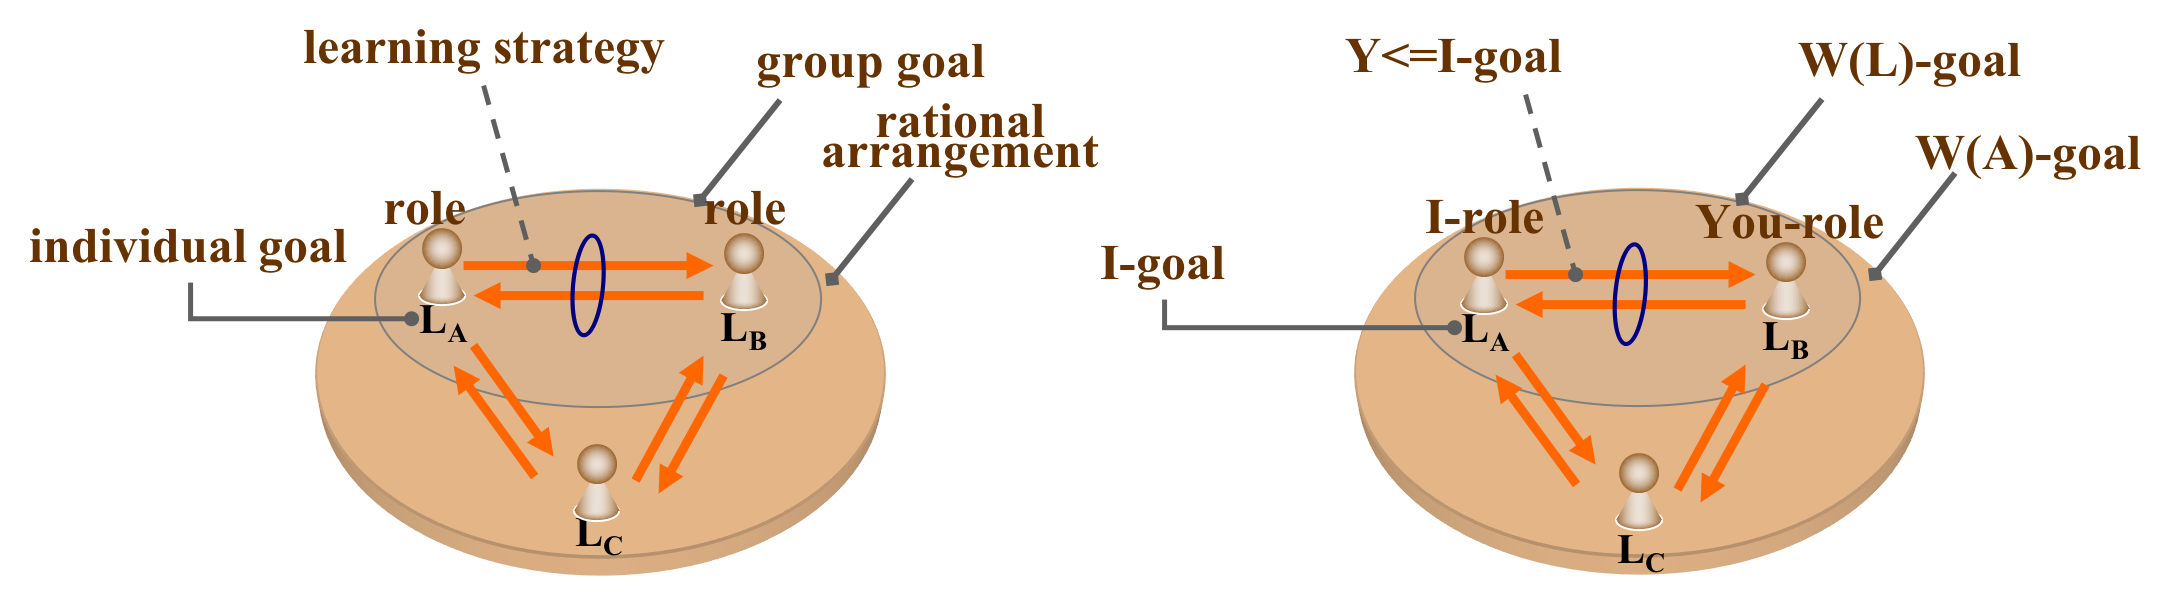
\includegraphics[width=0.95\textwidth]{images/chap-ontogacles1/concepts-terms-and-relation-in-cl-ontology.png}
 \fdireta{Isotani2009}
\end{figure}

To express the relationship of concepts described above, the CL Ontology employs the ontological structure shown in \autoref{fig:ontological-structure-cl-scenario} to represent CL scenarios. In this ontological structure, a CL scenario is composed by three parts defined as:  the \emph{Group structure benefit} (\emph{W(S)-goal}) to represent the expected benefits of the structured collaboration (i.e. positive interdependence, individual accountability, promotive interactions); the \emph{Learning strategy} (\emph{Y<=I-goal}) to represent the learning strategies employed by the group members in the CL scenario; and (3) the \emph{CL process} to represent the rational arrangement of the group activity (\emph{W(A)-goal}).

\begin{figure}[htb]
 \caption{Ontological structure to represent CL scenarios}
 \label{fig:ontological-structure-cl-scenario}
 \centering
 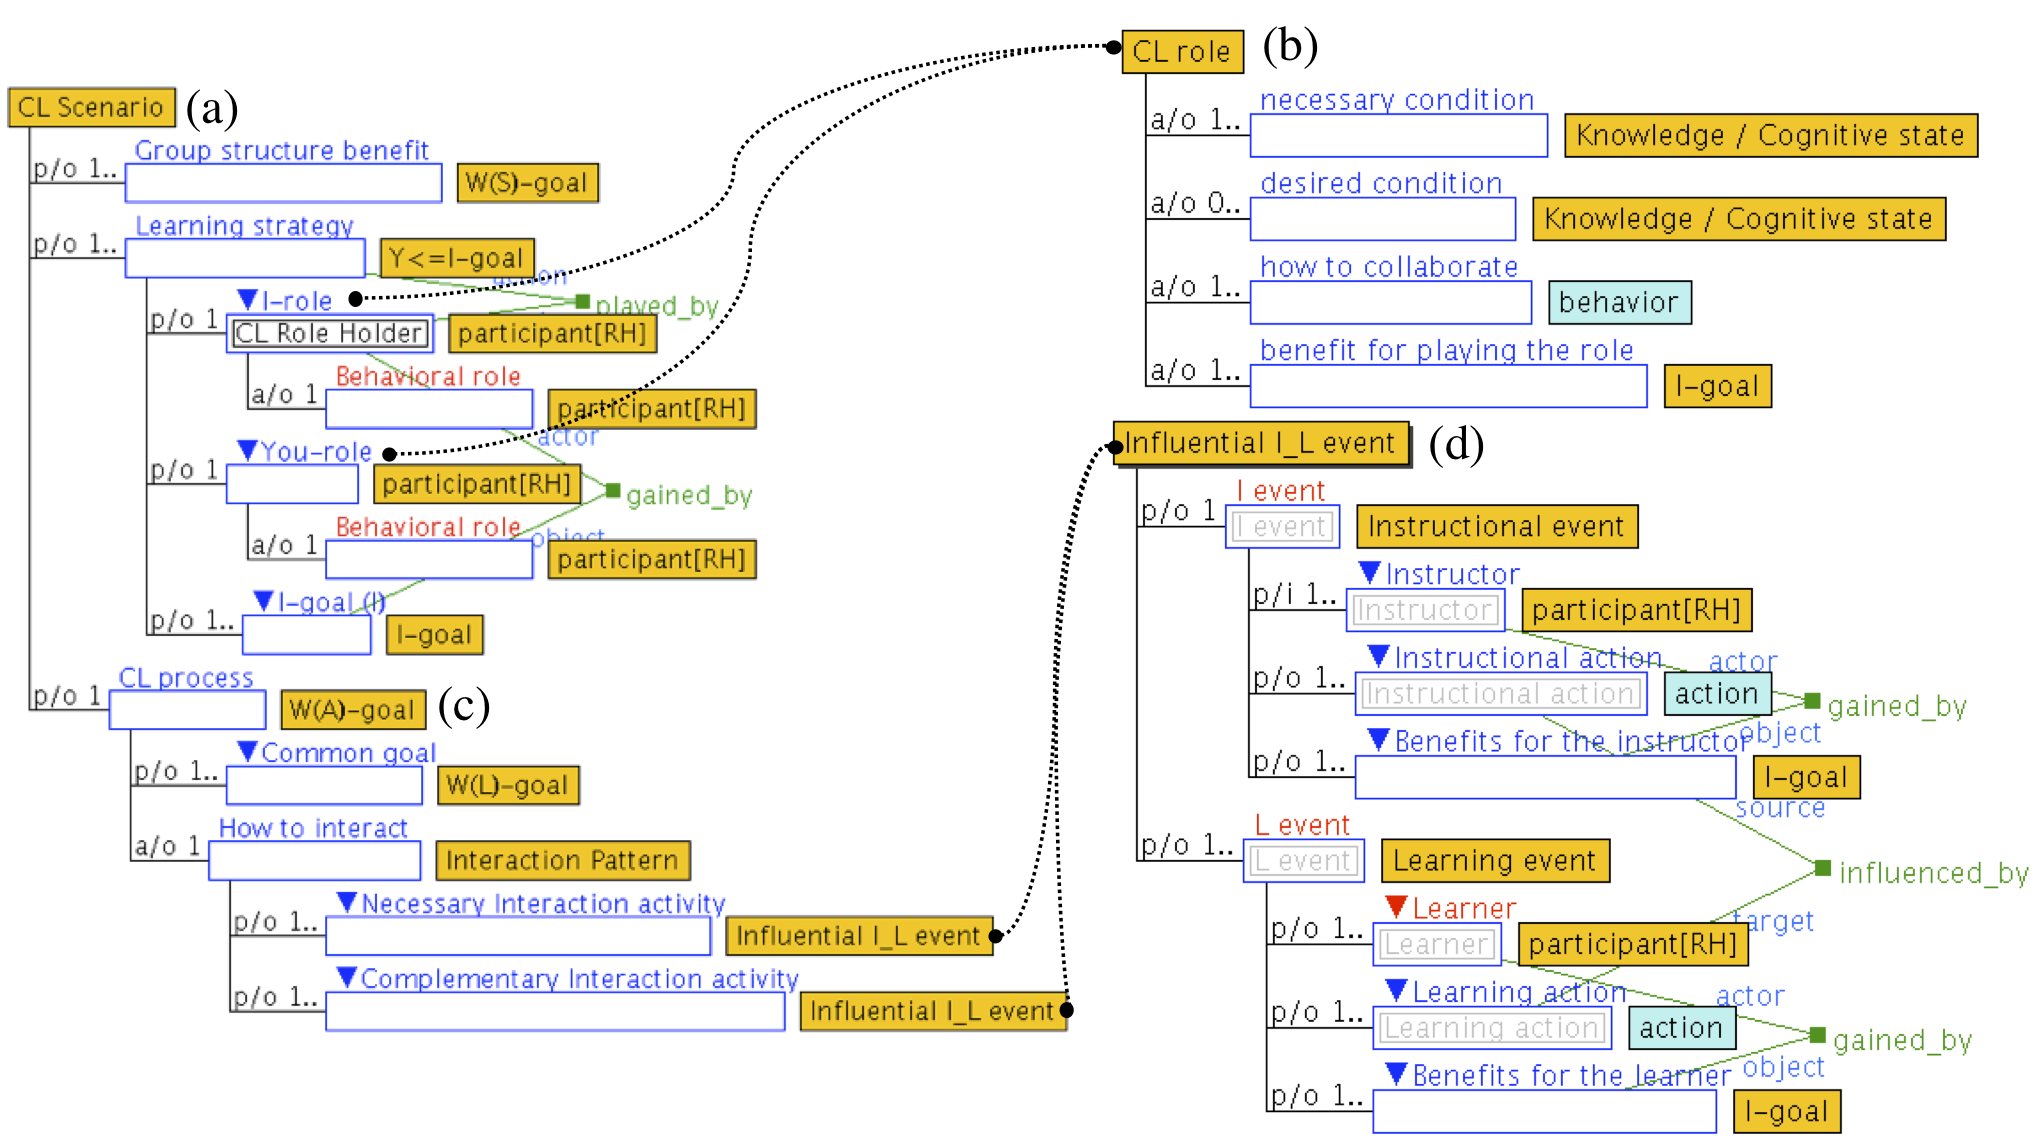
\includegraphics[width=1\textwidth]{images/chap-ontogacles1/ontological-structure-cl-scenario.png}
 \fdireta{Isotani2009}
\end{figure}

\begin{enumerate} [label=(\alph*)]

\item
The \textbf{Learning strategies} (\emph{Y<=I-goal}) are guidelines that specify how the participants should interact with others to achieve their individual goals. These guidelines help the group members to externalize a desired behavior to play a given CL role more adequately. Therefore, the Learning strategy is represented as an ontological structure composes by: the participant in focus (\emph{I}) who play a CL role (\emph{I-role}), the participant (\emph{You}) who interacts with the participant in focus (\emph{I}) playing a CL role (\emph{You-role}), and the individual learning goals (\emph{I-goal}) that are expected to be achieved by him/her at the end of CL scenario. The desired behaviors to be externalized by the group members  are represented in the ontological structure to represent \emph{Learning strategies} as part of the CL roles (\emph{I-role} and \emph{You-role}) in which these behaviors are expressed as a \emph{behavioral roles} to be played by a participant.

\item
The \textbf{CL role} consists functions, goals, duties and responsibilities that must be taken by the group members to achieve the common and individual learning goals. Thus, the ontological structure to represent a CL role describes: the \emph{necessary condition} and \emph{desired conditions} to play the role, \emph{how to collaborate} for playing the role, and the \emph{benefits for playing the role}. The current \emph{Cognitive/Knowledges states} of group members are used as necessary and desired conditions, the \emph{behaviors} describe \emph{how to collaborate} playing the role, and the expected \emph{benefits for playing the role} are expressed through individual learning goals (\emph{I-goal}).

\item
The \textbf{CL process} is the \emph{rational arrangement of group activity} (\emph{W(A)-goal}) whereby the common and individual learning goals are achieved by the group members. In this arrangement, the \emph{common learning goals} (\emph{W(L)-goal}) is the result of the negotiation process for the group formation, and the \emph{Interaction Pattern} is the sequencing mechanism whereby the participants will achieve their individual learning goals (\emph{I-goal}). This interaction pattern is represented as a set of \emph{necessary} and \emph{desired interactions} in which the interaction for the group members is defined as influential Instructional-Learning events (\emph{Influential I\_L events}).

\item
The \textbf{Influential I\_L event} explicitly represents the interaction among the group members and the benefits from two points of view: from the participants who play the role of instructor, and for the participants who play the role of learner. In the influential I\_L event, a group member performs actions and influences other members in the production of changes in the learning state helping them to achieve their individual learning goals. Therefore, the ontological structure to represent an influential I\_L event is composed by two events: a \emph{learning event} and an \emph{instructional event} in which there are represented the actors as participants of CL scenario playing CL roles and their actions. A participant in these event can act as an \emph{instructor} (participant who does an instructional action) or as a \emph{learner} (participant who does a learning action), and then, through the interactions among instructor, learner and learning objects, the attainment of educational benefits occurs. Thus, the ontological structure to represent an instructional event (\emph{I event}) and a learning event (\emph{L event}) consist in: a learner who plays the roles of \emph{Instructor}, a learner who plays the role of \emph{Learner}, the \emph{Instructional actions}, the \emph{Learning actions}, and the \emph{Benefits for the instructor} and \emph{Benefits for the learner}.
\end{enumerate}

As it was said before, the ontological structures presented in the \autoref{fig:ontological-structure-cl-scenario} are used to represent CL scenarios that compliant with instructional and learning theories. To illustrate this use, \autoref{fig:cognitive-apprenticeship-ontological-structure} shows the representation of CL scenario based on the Cognitive Apprentice theory. According to this theory, the CL activities should incorporate situations that are familiar to those who are using these activities, and these situations must to lead the participants to act and interact acquiring skills in a specific context, and then generalizing these skills to other situations. Therefore, the CL scenarios based on the Cognitive Apprentice theory focuses on supporting a more skilled participant, known as master, to teach a familiar situation for the lesser skilled participants known as apprentices, and then, the lesser skilled participants, known as apprentices, learn by observing the master's behavior and mimic it in other similar situations. Thus, from the viewpoint of the more skilled participant, he/she is supported by the learning strategy \aspas{\emph{learning by guiding}} (a1), his/her role (\emph{I-role}) is the \emph{Master role} with the behavioral role of \emph{Guider}, and his/her individual learning goals are the \emph{development of cognitive} or \emph{meta-cognitive skills} at the levels of \emph{Autonomous stage}. From the viewpoint of a lesser skilled participant, he/she is supported by the learning strategy \aspas{\emph{learning strategy by guiding}} (a2) to interact with the master, his/her role (\emph{I-role}) is the \emph{Apprentice role} with the behavioral role of \emph{Imitator}, and his/her individual goals are the \emph{development of cognitive} and/or \emph{meta-cognitive skills} at the levels of \emph{Cognitive stage} and \emph{Associative stage}.

\begin{figure}[htb]
 \caption{Ontological structure to represent CL scenario based on the Cognitive Apprenticeship theory}
 \label{fig:cognitive-apprenticeship-ontological-structure}
 \centering
 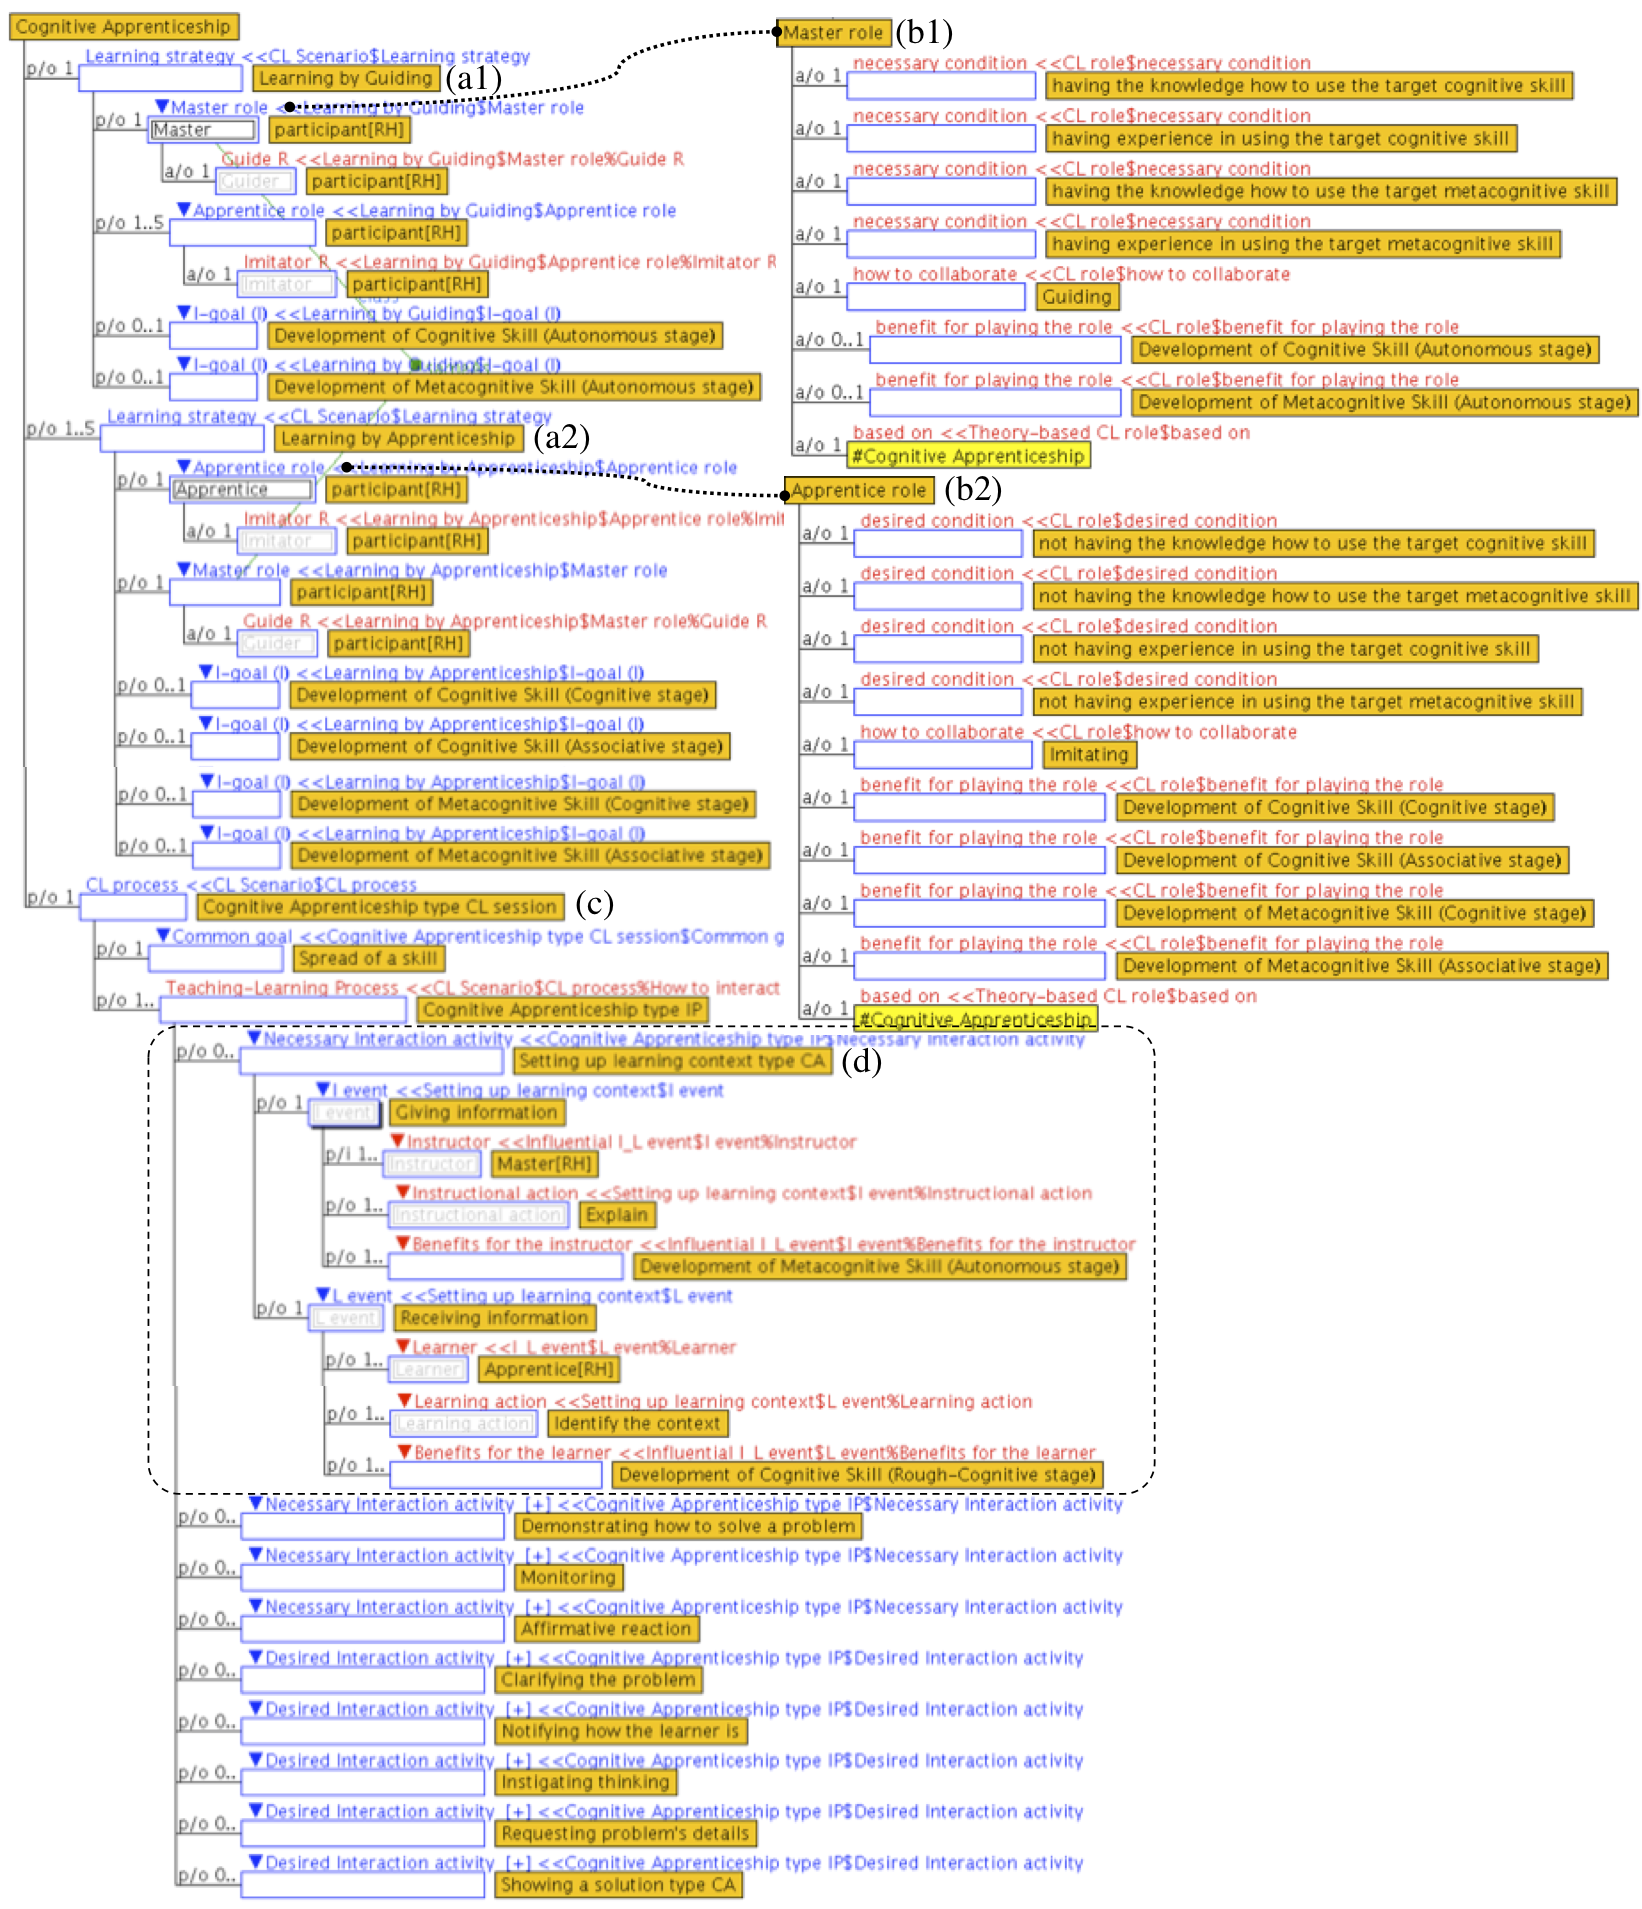
\includegraphics[width=1\textwidth]{images/chap-ontogacles1/cognitive-apprenticeship-ontological-structure.png}
 \fautor
\end{figure}

According to the Cognitive Apprentice theory, the necessary conditions to play the \emph{Master role} (b1) are: \emph{having the knowledge how to use the target cognitive skill}, \emph{having experience in using the target cognitive skill}, and/or \emph{having experience in using the target metacognitive skill}. If an participants adequately plays the role of master, he/she acts \emph{Guiding} to other participant to act or think similarly, and as consequence, he/she is benefited with the \emph{development of cognitive or metacognitive skill} to the \emph{Autonomous stage}. To play the \emph{Apprentice role} (b2), the Cognitive Apprenticeship theory indicates that the participants without any knowledge or experience in how to use the target skill should play the role of apprentice. Thus, there is not necessary conditions in the ontological structure shown in \autoref{fig:cognitive-apprenticeship-ontological-structure} (b2), and the desired conditions are \emph{not having the knowledge how to use target metacognitive or cognitive skill} and/or \emph{not having experience in using the target metacognitive or cognitive skill}. When a participant adequately play the \emph{Apprentice role}, he/she acts as \emph{Imitating} the behavior of the master participant and obtaining the benefits in the \emph{development of metacognitive or cognitive skill} at the levels of \emph{Cognitive stage} or \emph{Associative stage}.

When the two learning strategies, \emph{Learning by Guiding} and \emph{Learning by Apprenticeship}, are simultaneously employed to structure the interactions in the CL scenario, a positive synergy is created producing a \emph{spread of skills} across the group members. This arrangement is formalized in the ontological structure as shown in \autoref{fig:cognitive-apprenticeship-ontological-structure} (c), where the \emph{CL process} is a \emph{Cognitive Apprenticeship type CL session}, the \emph{Common goal} of this session is \emph{Spread of a skill}, and the \emph{Teaching-Learning Process} as an \emph{Interaction Pattern} is the sequencing mechanism defined by the CSCL scripts inspired by the Cognitive Apprenticeship theory shown in \autoref{fig:cognitive-apprenticeship-cscl-script}. To avoid all the details in the formalization of each \emph{Influential I\_L event} defined in the interaction pattern, only the structure to represent interaction \aspas{\emph{Setting up learning context type CA}} is shown with more detail in \autoref{fig:cognitive-apprenticeship-ontological-structure} (d). As shown in this formalization, in Instructional event \aspas{\emph{Giving Information}} (\emph{I event}), the participant who plays the role of \emph{Master} acts as an \emph{Instructor} doing the instructional action \aspas{\emph{Explain}} to achieve benefits in the \emph{Development of his/her metacognitive skill} at the level of \emph{Autonomous stage}. In the Learning event \aspas{\emph{Receiving information}} (\emph{L event}), the participant who acts playing the role of \emph{Learner} performs the learning action \aspas{\emph{Identify the context}} to obtain the benefits on the \emph{development of cognitive skill} at the level of \emph{Rough-Cognitive stage}.


\section{Modeling Gamified CL Scenarios}
\label{sec:modeling-gamified-cl-scenarios}

The concepts, terms and relations shown in \autoref{fig:concepts-terms-and-relation-in-gamified-cl-scenarios} have been formalized in the ontology OntoGaCLeS to represent a gamified CL scenario. These elements are independent from any theory and practice, and they are described as follows as:

\begin{description}
\item[\textbf{Y<=I-mot goal}]
is the \emph{individual motivational strategy} used to enhance the learning strategy (\emph{Y<=I-goal}) employed by a participant in focus (\emph{I}).

\item[\textbf{I-mot goal}]
is the \emph{individual motivational goal} for a participant in focus (\emph{I}), and it represents what is expected to happen in his/her motivational stage when an individual motivational strategy (\emph{Y<=I-mot goal}) is applied in the CL scenario to enhance the learning strategy (\emph{Y<=I-goal}) employed by the group members.

\item[\textbf{I-player role}]
is the \emph{player role} for a participant in focus (\emph{I}).

\item[\textbf{You-player role}]
is the \emph{player role} for a participant (\emph{You}) who interacts with the participant in focus (\emph{I}).

\item[\textbf{I-gameplay}]
is the \emph{individual gameplay strategy} for the participant in focus (\emph{I}), and it defines the implementation of individual motivational strategy (\emph{Y<=I-mot goal}) when this strategy is extracted from game design model or gamification models.
\end{description}

\begin{figure}[htb]
 \caption{Concepts, terms and relations defined in the ontology to represent gamified CL scenarios}
 \label{fig:concepts-terms-and-relation-in-gamified-cl-scenarios}
 \centering
 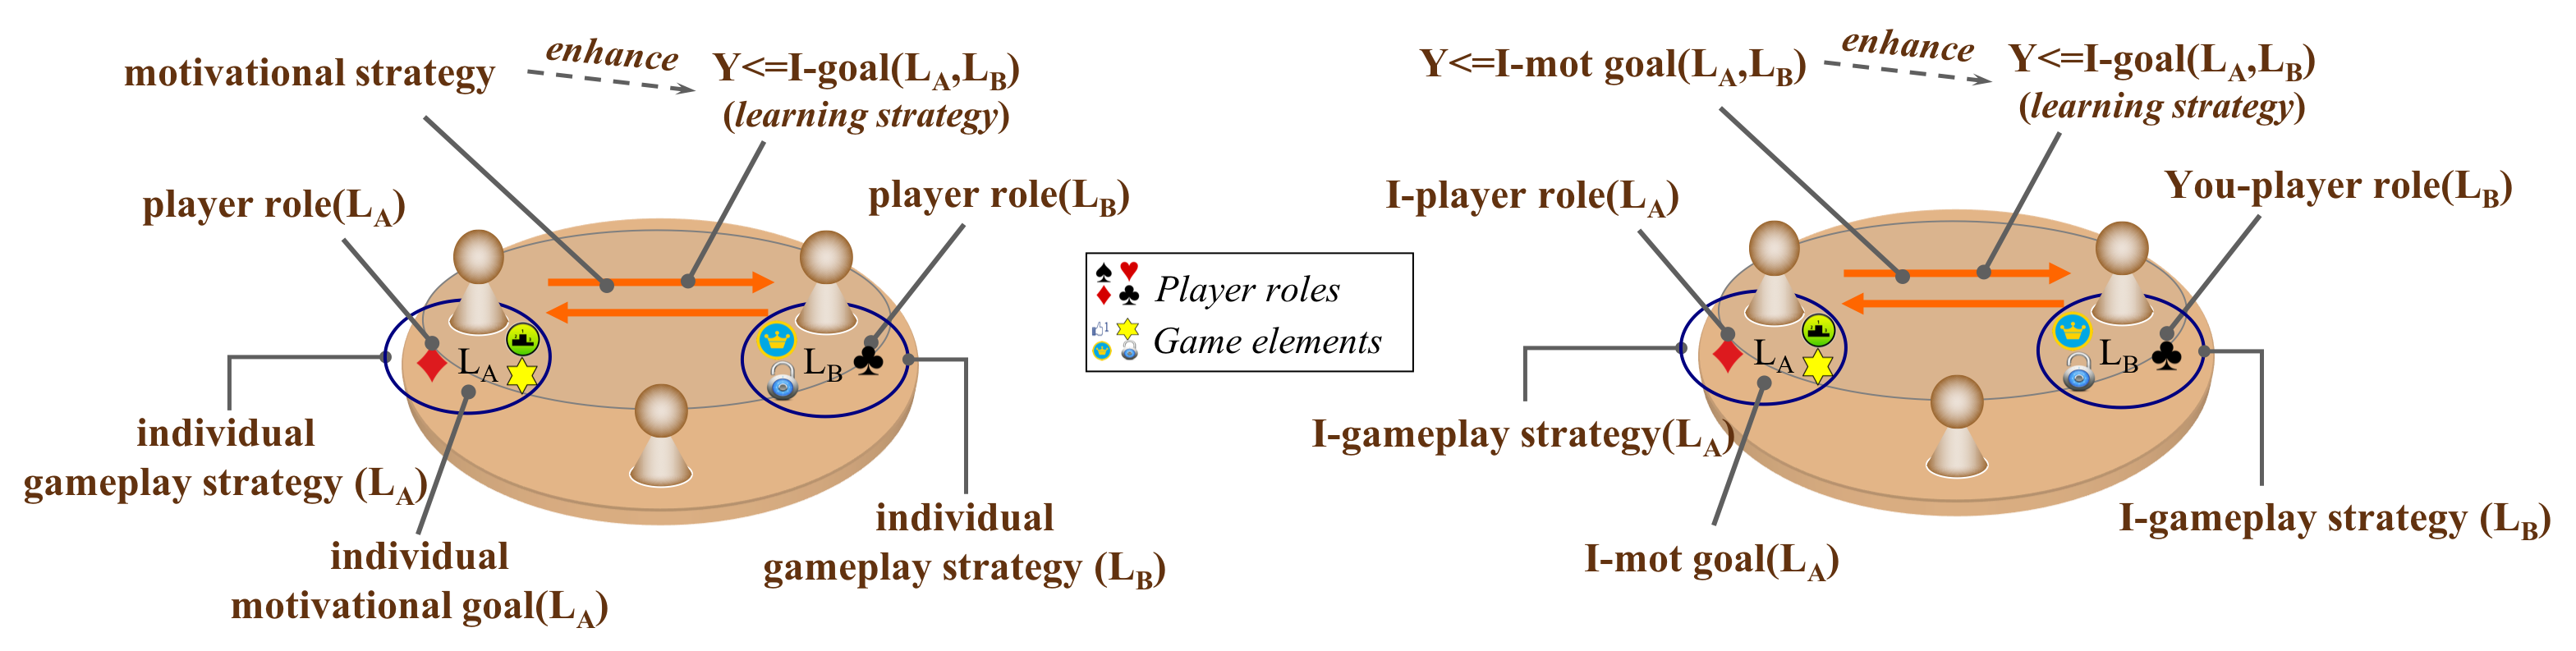
\includegraphics[width=1\textwidth]{images/chap-ontogacles1/concepts-terms-and-relation-in-gamified-cl-scenarios.png}
 \fautor
\end{figure}

In the following subsection, a detailed description related to the formalization of the concepts, terms and relation briefly described above are detailed.

\subsection{Individual Motivational Goal (I-mot goal)}
\label{subsec:individual-motivational-goal}

The \emph{individual motivational goal} (\emph{I-mot goal}) has been formalized in the ontology OntoGaCLeS to represent the reason why is necessary to apply an individual motivational strategy in a CL scenario. Thus, for a participant (\emph{I}) of CL scenario, the individual motivational goal (\emph{I-mot goal}) represents what it is expected to happen in his/her motivational stage when a motivational strategy is applied in the CL scenario to enhance the learning strategy employed by him/her to interact with others. In this sense, the individual motivational goal describes the motivational stages that must be reached by a person to be motivated to interact with other group members.

\autoref{fig:ontological-structure-i-mot-goal} shows the ontological structure that has been formalized in the ontology OntoGaCLeS to represent an individual motivational goal (\emph{I-mot goal}), where: the \emph{initial stage} and \emph{goal stage} are stages used to represent the expected change in the motivational stage of the person in focus (\emph{I}).

\begin{figure}[htb]
 \caption{Ontological structures to represent individual motivational goal (\emph{I-mot goal}). At the bottom, the \aspas{\emph{Satisfaction of psychological need}} (left) and the \aspas{\emph{Internalization of motivation}} (right)}
 \label{fig:ontological-structure-i-mot-goal}
 \centering
 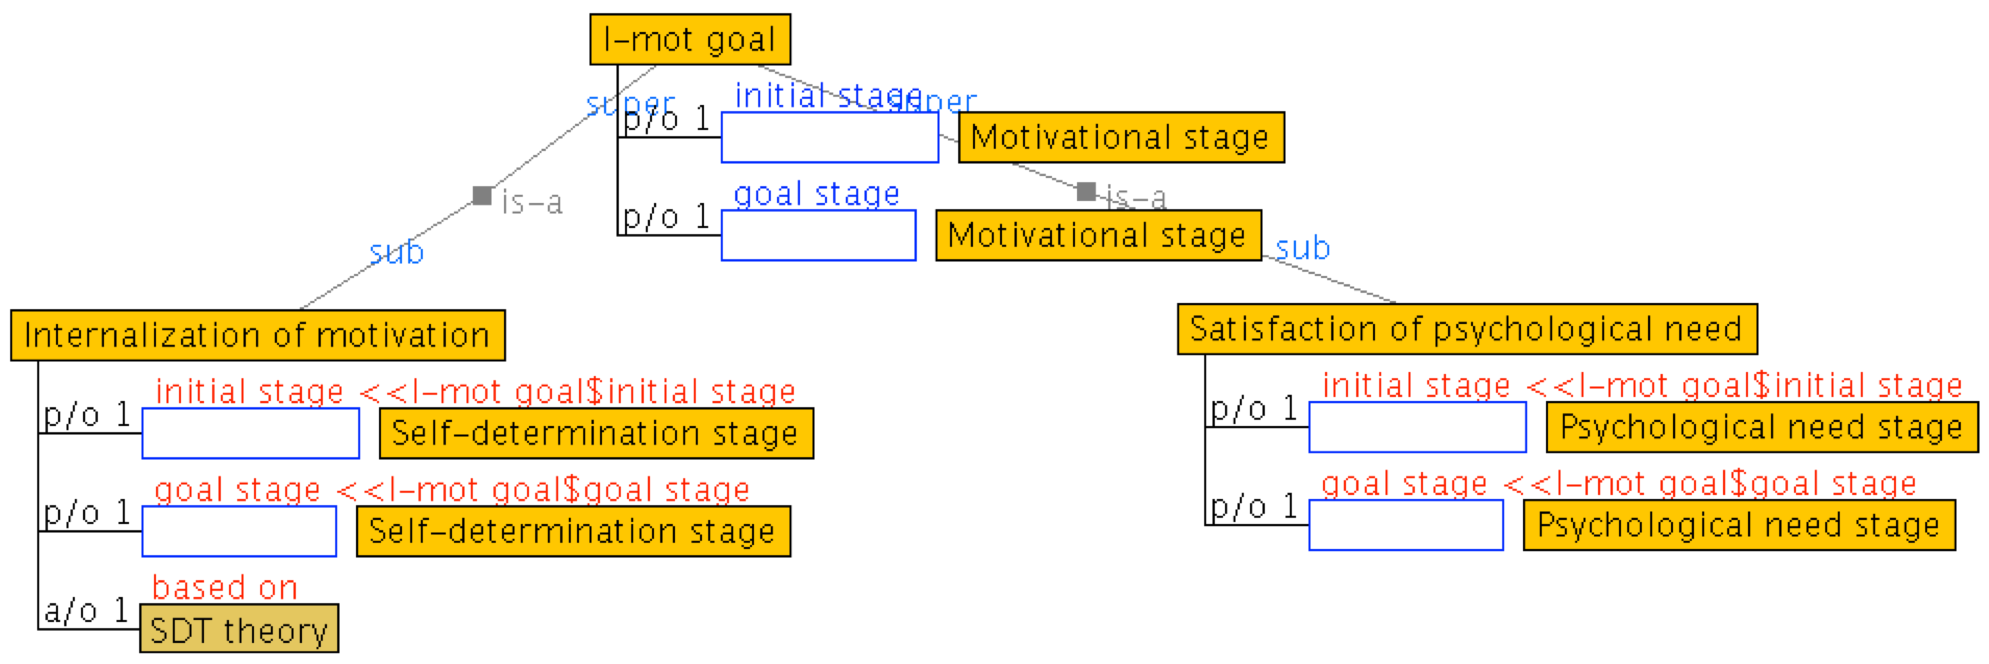
\includegraphics[width=1\textwidth]{images/chap-ontogacles1/ontological-structure-i-mot-goal.png}
 \fautor
\end{figure}

Two types of individual motivational goals have been currently formalized in the ontology OntoGaCLeS to describe the individual motivational goals (\emph{I-mot goal}) related to gamification as individual motivational strategy. The former know as \emph{Satisfaction of psychological needs} has been formalized based on the conceptualization of motivation as internal psychological process to satisfy human needs \cite{PritchardAshwood2008}, and the latter know as \emph{Internalization of motivation} has been formalized based on the form in which an individual regulates his own choices to behave and act \cite{DeciRyan2010}. \autoref{fig:ontological-structure-i-mot-goal} shows the current representation of these two type of individual motivational goals. The initial and goal stages related to the \emph{Internalization of motivation} are defined by the self-determination stage, whereas the initial and goal stages for the \emph{Satisfaction of psychological need} are defined by the \emph{psychological need stages}. In the articles  \cite{ChallcoMoreiraBittencourtMizoguchiIsotani2015, ChallcoMoreiraMizoguchiIsotani2014, ChallcoMoreiraMizoguchiIsotani2014a}, the author of this thesis has been used the term \aspas{\emph{Phychological need}} to refer the term \aspas{\emph{Psychological need stage}} used here, and the term \aspas{\emph{Without need}} to refer the group of terms described here as \aspas{\emph{\$1 need satisfied}} where \$1 is substitute for a psychological need (e.g. \emph{Mastery need satisfied}, \emph{Autonomy need satisfied}).

As it was mentioned before in the \autoref{sec:motivation-problem}, motivation is an internal psychological process associated with the three general components of arousal, direction and intensity dimension in which the arousal component is caused by needs (also called \emph{wants} or \emph{desires}). Such needs cause that a person behaves and acts to satisfy the needs \cite{MitchellDaniels2003}. Consequently, motivation describes how a person chooses to allocate time and energy to different behavior and actions to maximize the satisfaction of his own needs \cite{PritchardAshwood2008}. It means that, in a CL session, the motivation problem for the participant in focus (\emph{I}) occurs when he/she believes that the scripted collaboration will not lead him/her to satisfy his/her individual needs. Hence, the motivational strategy is introduced in the CL scenario to change this perception. Thus, the individual motivational goals (\emph{I-mot goal}) for the person in focus (\emph{I}) are the satisfaction of needs. More specifically, for the gamification of CL scenarios, the individual motivational goal is the \emph{Satisfaction of psychological needs} because game elements do not satisfy all human needs, they can only satisfy part of these needs that are referred by the thesis author as \emph{psychological needs}. The psychological needs are the human needs classified in the groups of relatedness and growth needs according to the ERG (Existence, Relatedness and Growth) theory \cite{Alderfer1972}.

\autoref{fig:ontological-structure-satisfaction-psychological-need} shows the ontological structures that had been formalized in the ontology OntoGaCLeS to represent the \emph{Satisfaction of psychological need} related to gamification as an individual motivational strategy. These ontological structures represent the satisfaction of innate psychological needs, and they comprise what is intended to evoke in minds of players by the majority of experts in gamification when a CL scenario is been gamified \cite{MoraRieraGonzalezArnedo-Moreno2015, SeabornFels2015}. According to the SDT theory, the well-being of an individual is reached when the psychological needs of autonomy, competence and relatedness are satisfied by performing a behavior \cite{DeciRyan1985, DeciRyan2010}, and according to the Dan Pink's theory \cite{Pink2011}, a person is motivate and engage in a cognitive, decision-making, creative or higher-order thinking task whether it is given with autonomy, mastery and purpose.

\begin{figure}[htb]
 \caption[Ontological structure to represent Satisfaction of psychological need]{Ontological structures to represent \aspas{\emph{Satisfaction of psychological need}} for gamification as motivational strategy. At the top right, the ontological structure to represent \aspas{\emph{Satisfaction of autonomy}.}}
 \label{fig:ontological-structure-satisfaction-psychological-need}
 \centering
 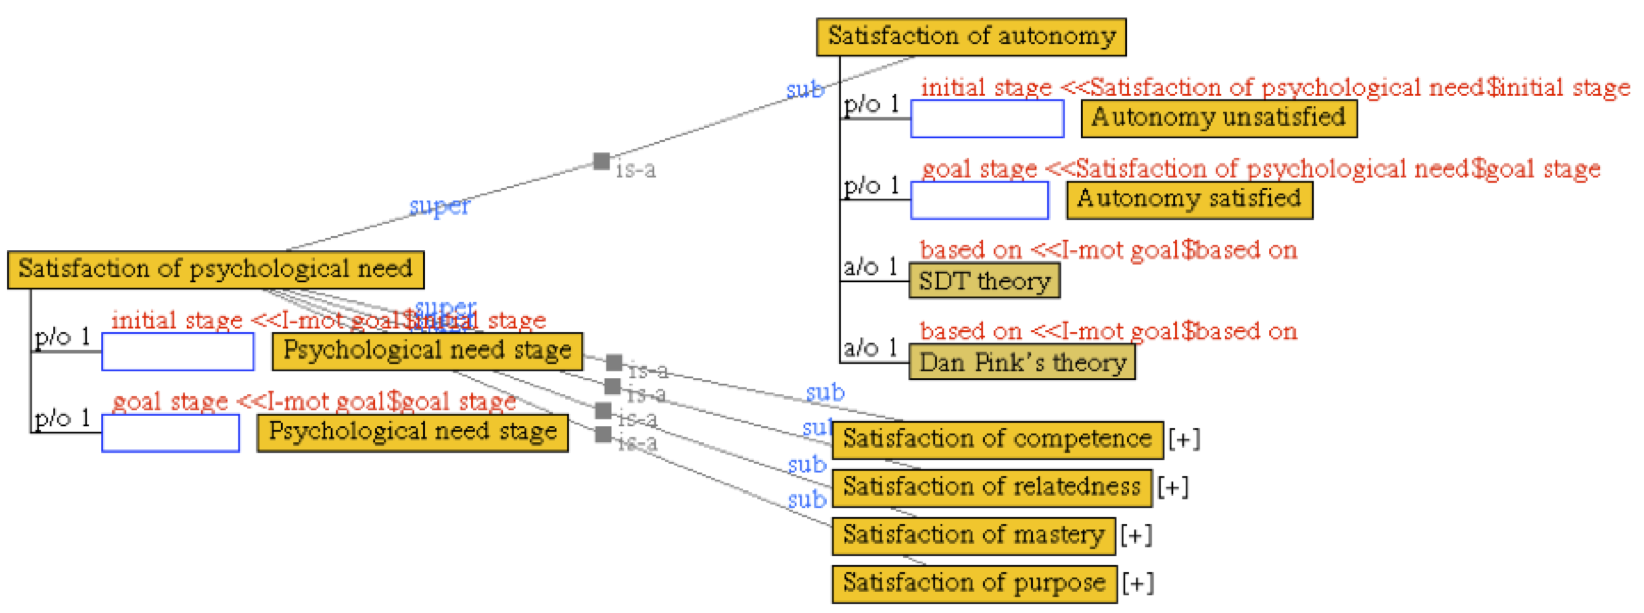
\includegraphics[width=1\textwidth]{images/chap-ontogacles1/ontological-structure-satisfaction-psychological-need.png}
 \fautor
\end{figure}

At the top right of \autoref{fig:ontological-structure-satisfaction-psychological-need}, the ontological structure to represent the \emph{Satisfaction of autonomy} is detailed in which, based on a unipolar scale of satisfaction from unsatisfied to satisfied needs, the roles of initial and goal stages are played by the \emph{Autonomy unsatisfied} and the \emph{Autonomy satisfied}, respectively. Employing the same unipolar scale, the satisfaction of four psychological needs have been formalized in the ontology OntoGaCLeS, and they are detailed in the \autoref{appendix:i-mot-goal}.

The \emph{internalization of motivation} is the process by which \aspas{\emph{values, attitudes, or regulatory structures, such that the external regulation of a behavior is transformed into an internal regulation, so no longer requires the presence of an external contingency}} \cite{GagneDeci2005}. In this sense, the internalization of motivation in relation to the satisfaction of needs refers to the change from a non-free choice to a free choice of needs that will be satisfied by oneself. According to the SDT theory \cite{DeciRyan1985, RyanDeci2000}, this change happens from the extrinsic motivation to intrinsic motivation when motivation is changed from a non-self-determined form (\emph{non-freely choice}) to a self-determined form (\emph{freely choice by oneself}). Here, instead to consider only as positive the creation of intrinsic motivation while the extrinsic motivation is treated as undesirable when a CL session is being gamified, the extrinsic motivators employed by the game elements must be used as an attempt to transform the current stage of students' motivation from amotivation and extrinsic motivation into intrinsic motivation.

\autoref{fig:ontological-structure-internalization-motivation} shows the ontological structures formalized in the ontology OntoGaCLeS to represent the \emph{Internalization of motivation} as individual motivational goal for a person in focus (\emph{I}) when gamification is applied as an individual motivational strategy. According to the SDT theory \cite{DeciRyan2010, DeciVansteenkiste2004}, this internalization happens on a continuum ranging of stages from \emph{amotivation} (not internalized behave) into \emph{external motivation} (not at all internalized behave) to \emph{introjected motivation} (partially internalized behave) to \emph{identified motivation} (fully internalized behave) to \emph{intrinsic motivation} (automatically internalized behave. Thus, this range of \emph{motivation stages} has been used to represent the initial and goal stages in the ontological structures to represent the internalizations of motivation as shown in \autoref{fig:ontological-structure-internalization-motivation}.

\begin{figure}[htb]
 \caption[Ontological structures to represent Internalization of motivation]{Ontological structures to represent \aspas{\emph{Internalization of motivation}} as individual motivational goal. At the top right, the structure to represent \aspas{\emph{Internalization from amotivation to intrinsic motion}.}}
 \label{fig:ontological-structure-internalization-motivation}
 \centering
 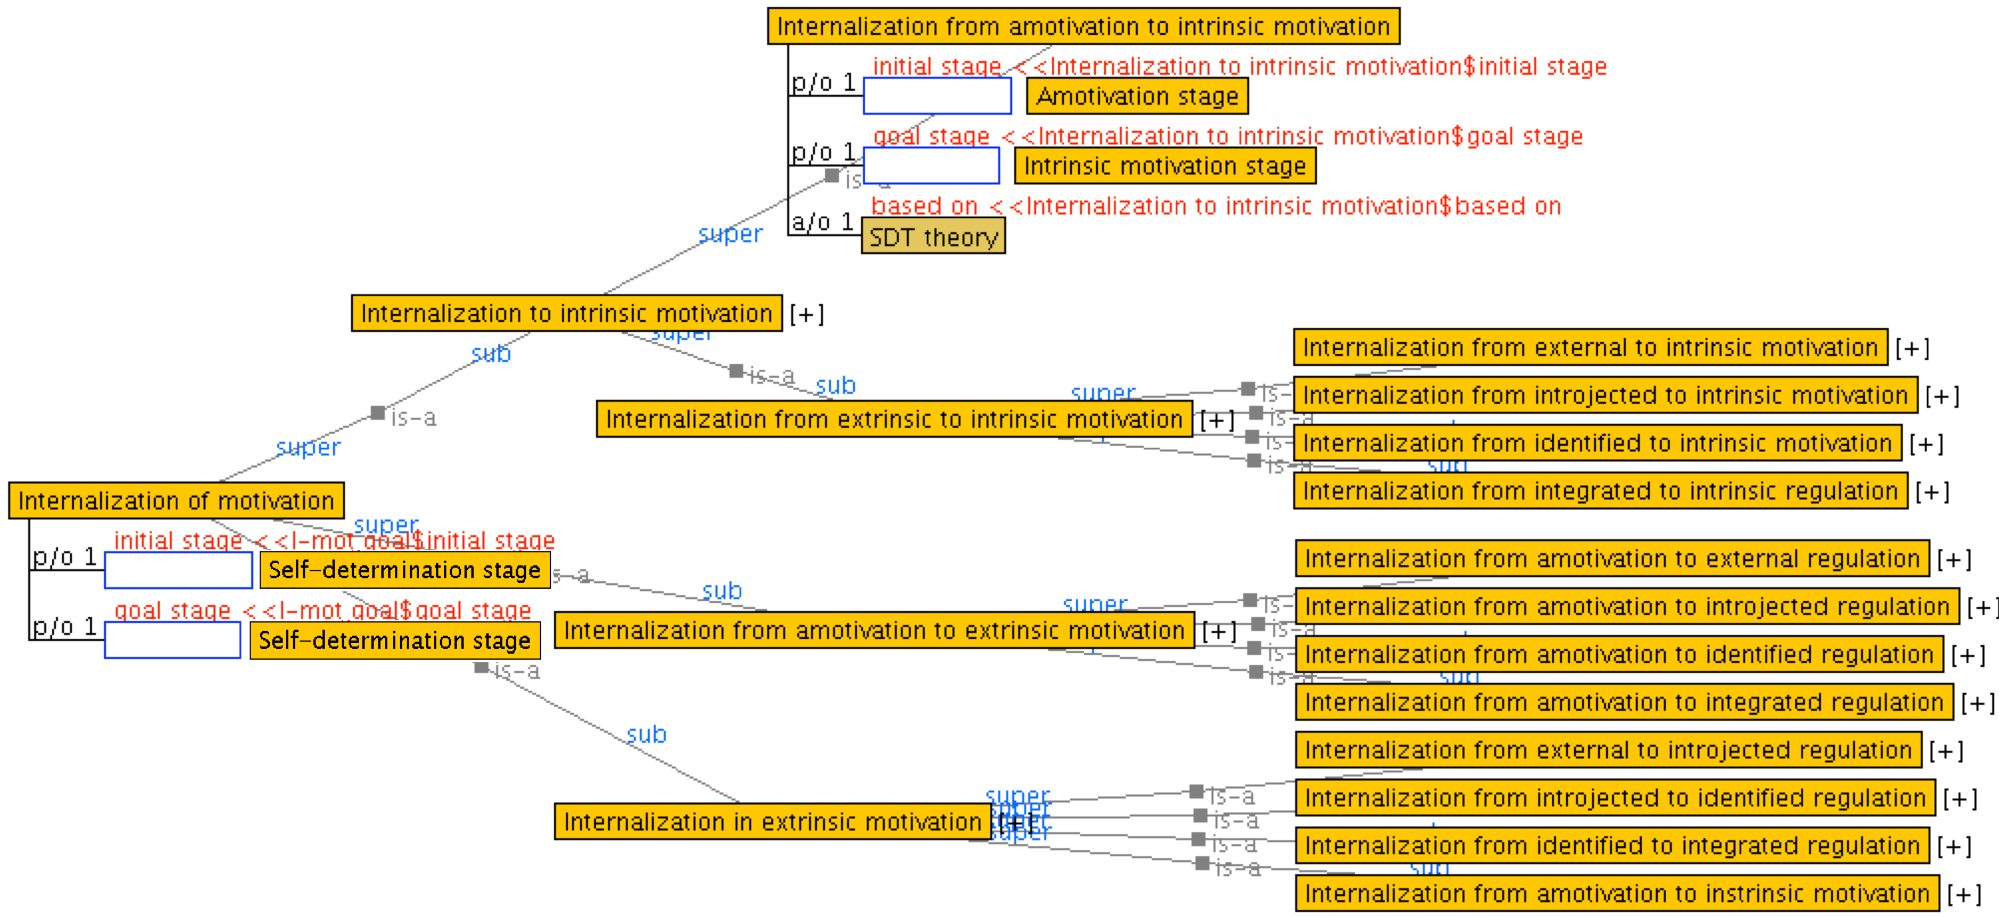
\includegraphics[width=1\textwidth]{images/chap-ontogacles1/ontological-structure-internalization-motivation.png}
 \fautor
\end{figure}

In the gamification of CL scenarios, the goal stage is always the \emph{intrinsic motivation stage} because the game elements are introduced in the CL scenario as an attempt to transform the current motivation stage, from amotivation or extrinsic motivation stage into intrinsic motivation stage (\emph{Internalization to intrinsic motivation}). Thus, for example, in the formalization of \emph{Internalization from amotivation to instrinsic motivation}, the initial stage is \emph{Amotivation stage} and the goal stage is \emph{Intrinsic motivation stage} as shown at the top right of \autoref{fig:ontological-structure-internalization-motivation}. Based on the range of motivation stage described by the SDT theory, we have formalized sixteen internalizations of motivation in the ontology OntoGaCLeS that are detailed in \autoref{appendix:i-mot-goal}.


\subsection{Player Role}
\label{subsec:player-role}

The identification of homogeneous people groups that differ from other groups in a significant way is essential to define the personalization in any system. In game design, this segmentation of the people is established by player types models in which player typologies categorize the players in different groups according to their geographic location \cite{BenJuddChrisAvelloneHideoKojimaKeijiInafune2016, ChakrabortyNorcioVeerAndreMillerRegelsberger2015}, their demographic situation \cite{GreenbergSherryLachlanLucasHolmstrom2010, Shaw2012}, their psychographic characteristic \cite{Tseng2011, Yee2006}, and their behavioral characteristics \cite{Bartle2004, Lazzaro2009}. These player type models aim to help the game development teams to identify the features that make a game fun, enjoyable and/or desirable for a particular audience. However, the player type models cannot be extrapolated to others types of games for which they were not intended, and the information provided by them cannot be directly used in the gamification of CL scenarios. Thus, the concept of \emph{Player role} has been defined in the formalization of gamified CL scenarios to describe player types.

The \emph{Player role} is the role that describes the functionality, responsibilities and requirements whereby a particular group of participants becomes players in a gamified CL scenario. This segmentation is based on individual characteristics that establish a segmentation of participants using necessary and desired conditions. In this sense, the \emph{Player role} has been formalized in the ontology OntoGaCLeS as the ontological structure shown in \autoref{fig:ontological-structure-player-role}. This structure defines the conditions that must be satisfied by a participant in the CL scenario to play the player role as: \emph{necessary condition} and \emph{desired condition}. Thus, a participant of CL scenario cannot play a player role if he/she does not fulfill the necessary conditions, and when the participant fulfills the necessary and desired conditions has more probability to obtain the expected \emph{benefits for playing the role}.

\begin{figure}[htb]
 \caption[Ontological structures to represent Player role]{Ontological structures to represent \aspas{\emph{Player role}} (At the top). At the bottom, the ontological structure to represent the player role of \aspas{\emph{Dreamer role}.}}
 \label{fig:ontological-structure-player-role}
 \centering
 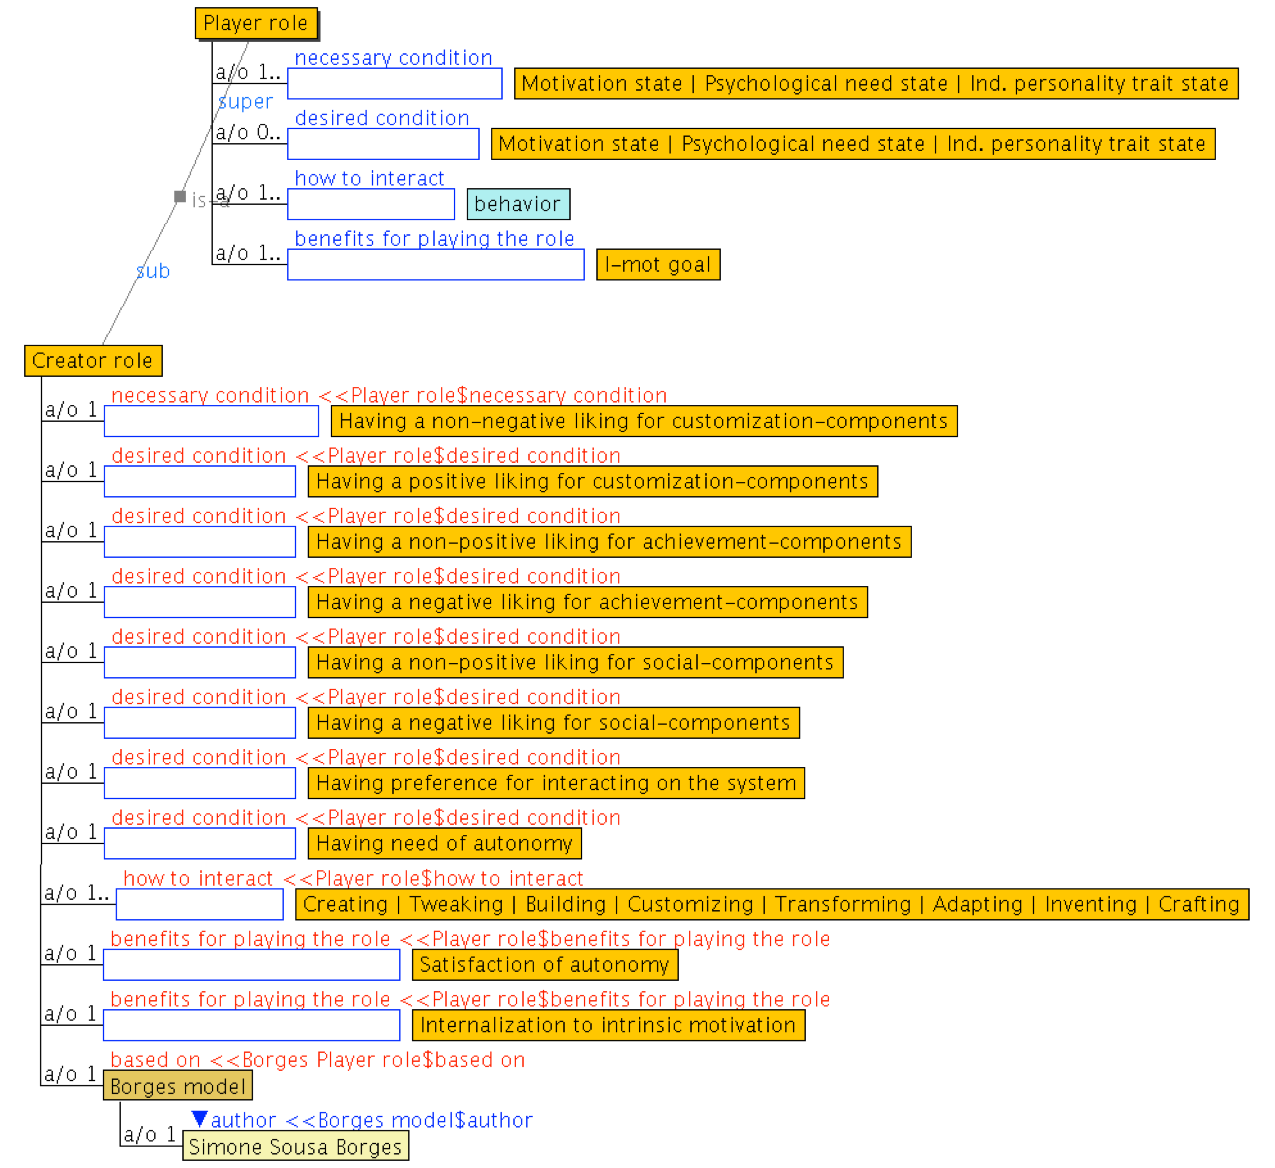
\includegraphics[width=1\textwidth]{images/chap-ontogacles1/ontological-structure-player-role.png}
 \fautor
\end{figure}

The necessary and desire conditions of a \emph{Player role} is represented using: motivation states, psychological need states, and individual personality trait states. \autoref{appendix:tree-overview-states} shows a tree overview for these states that have been currently formalized in the ontology OntoGaCLeS to represent the conditions in the \emph{Player roles}.

\begin{itemize}
\item
The \emph{Motivation state} is an internal state that describes the temporal attitudinal state of a person in relation to his/her desire to be a participant in the CL session. These stages can be \emph{Not motivated} and \emph{Motivated}. The state of motivated is also divided in two types: \aspas{\emph{Intrinsic motivated}} and \aspas{\emph{Extrinsic motivated}} \cite{DeciRyan2010}. It is important to notice here that the motivation state is not as same as motivation stage. Although both concepts represent changes in relation to the motivation, the motivation state represents a specific part of the whole process of being motivated, whereas the motivation stage represents an interval in the whole process of being motivated.

\item
The \emph{Psychological need state} is used to represent the current psychological needs of a person in which the states for each one of the psychological needs are formalized through the representation of pair states: \aspas{\emph{Having need of \$1}} and \aspas{\emph{Not having need of \$1}} where \aspas{\emph{\$1}} is replaced by the name of the need that is being described as prerequisite. For instance, to represent the states related to the psychological need of competence, the states \aspas{\emph{Having need of competence}} and \aspas{\emph{Not having need of competence}} have been formalized in the ontology OntoGaCLeS.

\item
The \emph{Ind, personality trait state} describes states related to individual personality traits, such as introversion, extraversion, openness to experience, and conscientiousness. The individual personality trait states describe the characteristic that make a person unique by indicating his habitual patterns of thought, emotion and behavior for different situations \cite{MatthewsDearyWhiteman2003}. These states express whether a participant either has or does not have the individual personality trait. These states also express the personality traits in a rating of dimensions, e.g. extraversion vs introversion. Currently, the ontology OntoGaCLeS represents the individual personality traits states related to: the big five personality traits \cite{CostaMacCrae1992}, the MBTI personality traits \cite{Briggs1976}, the game-playing style preferences described in the Bartle's player type model \cite{Bartle2004}, and the game-playing liking preferences described in the Yee's motivation components \cite{Yee2006} (\autoref{ appendix:tree-overview-states}).
\end{itemize}

The ontological structure to represent \emph{Player role} shown in \autoref{fig:ontological-structure-player-role} also includes the information about: how the participant with the player role is expected to interact with the game elements (\emph{how to interact}), and the expected benefits for playing the player role (\emph{benefits for playing the role}). The \emph{behavior} indicates the possible manners in which a participant should interact playing the player role to attain the expected \emph{benefits for playing the role}. These benefits are represented as \emph{individual motivational goals} (\emph{I-mot goal}).

At the bottom of \autoref{fig:ontological-structure-player-role}, the \emph{Creator role} is shown as example of the formalization of a player role using the ontological structures proposed in this section. According to this structure, participants who have a greater liking for customization-components rather than for other game components are classified as creators. This segmentation is represented by the necessary condition of \emph{having a non-negative liking for customization-components}, and the desired conditions of \emph{having a positive liking for customization-components}, \emph{having a non-positive liking for achievement-component}, \emph{having a negative liking for achievement-component}, \emph{having a non-positive liking for social-component}, and \emph{having a negative liking for social-component}. The desired conditions related to the behavioral characteristics are: \emph{having preference for interacting on the system} and \emph{having need of autonomy}. The expected behaviors to obtain the benefits for playing the creator role are: \emph{Creating}, \emph{Tweaking}, \emph{Building}, \emph{Customizing}, \emph{Transforming}, \emph{Adapting}, \emph{Inventing} or \emph{Crafting}. As consequence of this behave, it is expected that the participants attain the \emph{Satisfaction of autonomy} and the \emph{Internalization to intrinsic motivation} (\emph{I-mot goal}).

In the ontology OntoGaCLeS, based on the information extracted from five different player type models, twenty-six players roles have been formalized and represented using the ontological structure proposed in this section. These player roles, their conditions, expected behaviors and benefits for the person who plays the role are detailed in the \autoref{appendix:player-role}.

\subsection{Individual Motivational Strategy (Y<=I-mot goal)}

In the context of CL scenarios, an \emph{individual motivational strategy} is defined by the thesis author as a set of guidelines defined to motivate a participant to interact with other group member using a learning strategy. These guidelines are independent of any technology, so that the individual motivational strategy describes what motivates a participant to act and behave in certain way. For example, consider the following guidelines extracted from the Model-driven Persuasive Game in which:

\begin{citation}
\aspas{cooperation is only a significant motivator of behaviour change for achievers and socializers, with ($\beta$=.15) and ($\beta$=.17) respectively. This is in line with the gaming style of socializers, who enjoy helping others. Achievers would also prefer to cooperate because they are inherently more altruistic ... achievers do often co-operate with one another, usually to perform some difficult collective goal, and from these shared experiences can grow deep, enduring friendships which may surpass in intensity those commonly found among individuals other groups.} \citeonline{Orji2014}.
\end{citation}

When these two guidelines are applied in a CL scenario by providing a situation in which the participants must cooperate to achieve a group goal (e.g. obtain a especial reward based on the collective performance of group members), these guidelines becomes a individual motivational strategy that could be applied to motivate participant who fall in the category of socializer or achiever because they are motivated by the desired to accomplish the group goal and the desired to help others, respectively.

For the formalization of individual motivational strategies whose guidelines are extracted from game design models or gamification models, the ontological structure shown in \autoref{fig:ontological-structure-individual-motivational-strategy} has been proposed by the thesis author. According to this structure, an \emph{individual motivational strategy} (\emph{Y<=I-mot goal}) describes:

\begin{description}
\item[\textbf{I-player role}]
as the participant in focus (\emph{I}) as a \emph{player role holder} who is motivated by the motivational strategy.

\item[\textbf{You-player role}]


\item[\textbf{I-mot goal (I)}]

\end{description}

the participant are \emph{player roles}, and the reasons why the participants are motivated by this strategy are expressed as \emph{individual motivational goal}. According to this structure, an \emph{individual motivational strategy} (\emph{Y<=I-mot goal}) describes the following elements:

\begin{description}
\item[\textbf{I-player role}] 
to indicate the \emph{player role holder} for the participant in focus (\emph{I}), and the \emph{behavioral roles} whereby this participant is motivated to interact with other participant (\emph{You}) using a learning strategy (\emph{Y<=I-goal}).


\item[\textbf{You-player role}]


\item[\textbf{I-mot goal}]

\end{description} 

ontology OntoGaCLeS


 that is extracted from game design model or gamification models, their 



 cooperative situation in which a participant who plays the socializer or achiever role must to help others, and the achiever 





 that motivates a participant in focus (\emph{I}) to use the learning strategy (\emph{Y<=I-goal}) during his/her interaction with other group member (\emph{You}), this guideline becomes an individual motivational strategy.



As is shown in the example , these guidelines are extracted from game design or gamification models, they consist in the description about how players types are motivated to perform behaviors in a specific situation, and the reason why they are motivated to perform these behaviors. For example, in 


In a CL scenario, for the participant in focus (\emph{I}) who interacts with other participant (\emph{You}) employing a learning strategy (\emph{Y<=I-goal}), an \emph{Individual motivational strategy} (\emph{Y<=I-mot goal}) is defined as the strategy that, independently of any technology, causes effects on motivation to interact with other group members using the learning strategy (\emph{Y<=I-goal}).


As we see in  example presented above, the individual motivational strategies extracted from game design models consist in a 

 In the first example, the behavior to motivate socializers is helping others in a cooperative situation because they like to help others. In the second example, the guidelines indicates that, in cooperative situation, achievers are motivated to collaborate with other participant when there is a difficult collective goal to be achieved. Thus, the ontological structure that has been formalized in the ontology OntoGaCLeS to represent individual motivational strategies extracted from game design models and gamification models is shown in \autoref{fig:ontological-structure-individual-motivation-strategy}, and it consists in:

\begin{itemize}
\item


\item
The player role (\emph{You-player role}) for the participant (\emph{You}) who interacts with the participant in focus (\emph{I}), and the \emph{behavioral roles} through which this participant is motivate to support the interaction of participant in focus (\emph{I}) using a learning strategy (\emph{Y<=I-goal}).

\item
The individual motivational goals (\emph{I-mot goal (I)}) whereby the participant in focus (\emph{I}) is motivated to interact with the other participant (\emph{You}) employing a learning strategy (\emph{Y<=I-goal}). In this sense, the individual motivational goals “\emph{I-mot goal (I)}” describe the reasons why the guidelines from a game design model or/and gamification model are applied as individual motivation strategy to enhance the learning strategy (\emph{Y<=I-goal}) employed by the participant in focus (\emph{I}) to interact with other participant (\emph{You}).
\end{itemize}

\begin{figure}[htb]
 \caption[Ontological structure to represent Individual motivational strategy]{Ontological structure to represent \aspas{\emph{Individual motivational strategy}} (at the left). At the right-top, the motivational strategy \aspas{\emph{Gamifying for Consumer and Dodecad Achiever}.} At the right-bottom, the motivational strategy \aspas{\emph{Gamifying by COOP}.}}
 \label{fig:ontological-structure-individual-motivational-strategy}
 \centering
 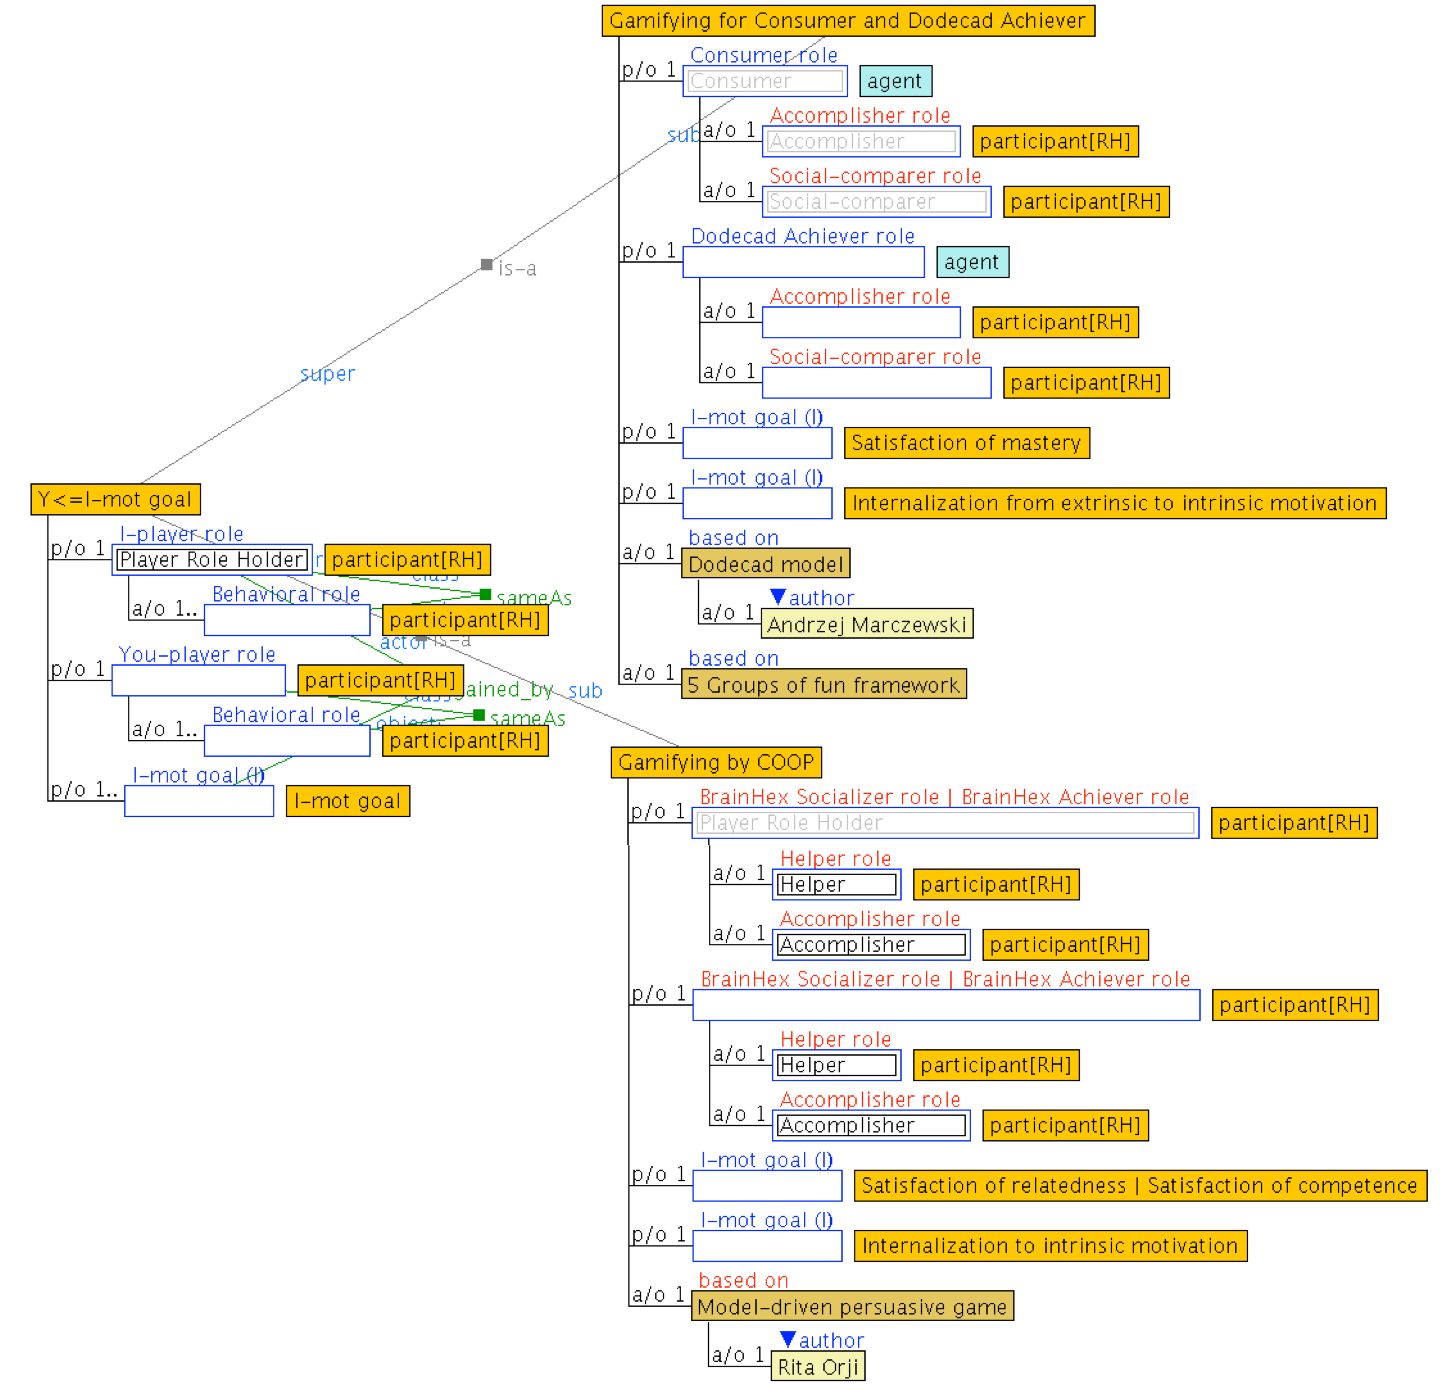
\includegraphics[width=1\textwidth]{images/chap-ontogacles1/ontological-structure-individual-motivational-strategy.png}
 \fautor
\end{figure}

To exemplify the formalization of the individual motivational strategies using the ontological structure proposed in this section, \autoref{fig:ontological-structure-individual-motivational-strategy} shows two examples in which the attribute \aspas{\emph{based on}} indicates the game design models and/or gamification model in which the motivational strategy (\emph{Y<=I-mot goal}) is based. The individual motivational strategy shown at the top-right of \autoref{fig:ontological-structure-individual-motivational-strategy} is known as \emph{Gamifying for Consumer and Dodecad Achiever}, and it has been formalized based on the guidelines of Dodecad model and 5 Groups of fun framework proposed by \citeonline{Marczewski2015a, 2015b}. According to these guidelines, the Consumers and Achievers are motivated by the need to obtain rewards that demonstrate for others their accomplishments in the domain of something. Hence, the behavioral roles of \emph{Accomplisher} and \emph{Social-comparer} are roles whereby a participant in focus (\emph{I}) playing the \emph{Consumer role} is motivated to interact with other participant (\emph{You}) who plays the \emph{Achieve role}. The \emph{Satisfaction of mastery} and the \emph{Internalization from extrinsic to intrinsic motivation} have been formalized as individual motivational goals for this individual motivational strategy because a consumer has the desired to demonstrate his/her mastery, and because the motivational strategy applied is in the CL scenario to turn the current extrinsic motivation of consumer into intrinsic motivation.

At the bottom-right of \autoref{fig:ontological-structure-individual-motivational-stratagy}, it is shown the ontological structure to represent the motivational strategy \aspas{\emph{Gamifying by COOP}.} This formalization has been based on the guidelines of Model-driven persuasive game \cite{OrjiVassilevaMandryk2014} in which, the cooperation is indicated as a significant motivator for socializers and achievers who enjoy helping others and cooperate with others in order to accomplish a difficult collective goal. Thereby, the behavioral roles for the participant in focus (\emph{I}) who play the \emph{BrainHex Socializer role} or \emph{Brainhex Achiever role} are either the \emph{Helper} and the \emph{Accomplisher}. Thus, the participant in focus (\emph{I}) will be to motivated to interact with other participant (\emph{You}) by his/her desire to accomplish the \emph{Satisfaction of relatedness} or the \emph{Satisfaction of competence}. As consequence of the cooperation, it is expected changes in the motivational state of participant in focus (\emph{I}) from the amotivation or extrinsic motivated state to the intrinsic motivated state (\emph{Internalization to intrinsic motivation}).

\autoref{appendix:ind-motivational-strategy} shows the individual motivational strategies for gamification currently defined in the ontology OntoGaCLeS, their player roles, their behavioral roles, and their individual motivational goals.

